\definizione{
Data $ f: I\to \R $, $ f $\marginnote{1 dic 2021} derivabile in $ I\setminus \{x_0\} $, $ f $ continua in $ x_0 $, se \[
    \lim_{x\to x_0} f'(x) = \pm \infty
\]
allora $ x_0 $ è un \textit{flesso a tangente verticale}.

In $ x_0 $ la tangente al grafico è verticale}
\esempio{}{
    $ f(x)=\sqrt[3]{x} $, derivabile in $ \R\setminus\{0\} $ \[
        f'(x)_{x\neq 0}=\frac{1}{3\sqrt[3]{x}} \xrightarrow[x\to 0]{} +\infty \displaystyle
    \]
}

\definizione{
    Data $ f: I\to \R $, $ f $ derivabile in $ I\setminus \{x_0\} $, $ f $ continua in $ x_0 $, se \[
    \lim_{x\to x_0^{+}} f'(x) = + \infty\:\land\: \lim_{x\to x_0^{-}} f'(x) = - \infty
\]
oppure
\[
    \lim_{x\to x_0^{+}} f'(x) = - \infty\:\land\: \lim_{x\to x_0^{-}} f'(x) = + \infty
\]
allora $ x_0 $ è detto \textit{cuspide}.
}{}

% FOTO 2

\section{Teoremi per le funzioni derivabili}

\subsection{Teorema di Fermat}

\esempi{}{
    \begin{enumerate}
        \item La funzione 
        
        \begin{center}
            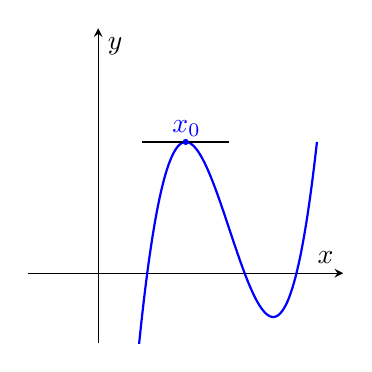
\begin{tikzpicture}
                \begin{axis}[
                xlabel=$x$,
                ylabel=$y$,
                axis equal,
                axis lines=middle,
                enlargelimits,
                xmax=5,
                xmin=-1,
                ymax=5,
                ymin=-1,
                xtick={0},
                ytick={0},
                scale only axis, 
                height=4cm, 
                width=4cm
                ]
            \addplot [blue, no marks, thick, domain=0:5, samples=1000] {(x-3)^3-3*x+10};
            \node at (2.02, 3.3) {\textcolor{blue}{$x_0$}};
            \addplot [thin] coordinates {(1, 3) (3,3)};
            \fill [blue] (2, 3) circle (0.07);
            \end{axis}
            \end{tikzpicture}
        \end{center}
        presenta in $ x_0 $ un punto di massimo locale; $ f $ è derivabile in $ x_0 $, e in questo punto la tangente è orizzontale.
        \item Per la funzione 
        \begin{center}
            \begin{tikzpicture}
                \begin{axis}[
                xlabel=$x$,
                ylabel=$y$,
                axis equal,
                axis lines=middle,
                enlargelimits,
                xmax=5,
                xmin=-1,
                ymax=5,
                ymin=-1,
                xtick={0},
                ytick={0},
                scale only axis, 
                height=4cm, 
                width=4cm
                ]
            \addplot [blue, no marks, thick, domain=0:5, samples=1000] {-sqrt(abs(x-1))+2};
            \node at (1.02, 2.3) {\textcolor{blue}{$x_0$}};
            \addplot [thin] coordinates {(0, 2) (2,2)};
            \fill [blue] (1, 2) circle (0.07);
            \end{axis}
            \end{tikzpicture}
        \end{center}
        $ x_0 $ è punto di massimo locale, ma la tangente in $ x_0 $ non è orizzontale perché non esiste.
    \end{enumerate}
}

\teorema[(di Fermat)]{difermatalleluia}{Se
    \begin{enumerate}
        \item $ f:I\to \R $, $ I $ intervallo;
        \item $ x_0 \in \mathring{I} $;
        \item $ x_0 $ punto di massimo o minimo locale;
        \item $ f $ derivabile in $ x_0 $;
    \end{enumerate}
    allora $ f'(x_0)=0 $, ovvero $ f $ ammette in $ x_0 $ tangente orizzontale.
}
\definizione{}{
    $ x_0 $ tale che $ f$ è derivabile in $ x_0 $ e $ f'(x_0)=0$ è detto \textit{punto critico} o \textit{stazionario} per $ f $.
}
\dimostrazione{difermatalleluia}{
    Studiamo il caso in cui $ x_0 $ punto di \textit{massimo} locale: \begin{equation}
        \exists\, U(x_0)\,\tc\quad \forall\,x \in U(x_0)\quad f(x)\le f(x_0)\: \bigl(\iff\, f(x)-f(x_0)\le 0\bigr)\label{eccociqui}
    \end{equation}
    Calcoliamo il limite: $\displaystyle
        \lim_{x\to x_0} \frac{f(x)-f(x_0)}{x-x_0}$: ci sono due casi.
    \begin{itemize}
        \item [(+)] Se $ x>x_0 $ \[
            \lim_{x\to x_0} \frac{f(x)-f(x_0)}{x-x_0} \underset{\footnotemark}{=}f'(x_0)\footnotetext{poiché $ f $ è derivabile in $ x_0 $}
        \]
        Vale inoltre $ f'(x_0)\le 0 $, per il teorema di permanenza del segno: infatti, nota \eqref{eccociqui}, si ha $ x-x_0>0 $.
        \item [(-)] Se $ x<x_0 $ \[
            \lim_{x\to x_0} \frac{f(x)-f(x_0)}{x-x_0} =f'(x_0)
        \]
        Inoltre $ f'(x_0)\ge 0 $ per il teorema di permanenza del segno: infatti, nota \eqref{eccociqui}, si ha $ x-x_0<0 $.
    \end{itemize}
    Allora deve essere \[
        f'(x_0)\le 0\:\land\: f'(x_0)\ge 0 \,\implies\, f'(x_0)=0
    \] %DOMANDA non mi piace questa dimostrazione, usare anche quella della piovano
}

\attenzione{
    Non vale il viceversa: un punto stazionario non implica un massimo (o un minimo).
}
\esempio{}{
    Sia $ f(x)=x^{3} $, $ \dom f=\R $: $ \forall\, x $, $ x \in \mathring{\R}$

    $ f'(x)=3x^{2} $, e $ f'(x)=0 $ $ \iff $ $ x=0 $, ma $ x_0=0 $ non è punto di massimo o minimo locale per $ f $. 

    $ x_0=0 $ è un flesso a tangente orizzontale\footnote{\hyperref[flesso]{definizione successiva}}.
}

\attenzione{Se $ x_0 $ è stazionario per $ f $, non è detto che sia massimo, minimo, o flesso a tangente orizzontale.}
\esempio{}{\label{esempiosinxquadrp}
    Data $ f(x)=\begin{cases}
        x^{2}\,\sin \frac{1}{x} & x\neq 0\\
        0 & x=0
    \end{cases} $ abbiamo verificato che $ f $ è derivabile in $ x_0=0 $, e $ f'(0)=0 $. $ x_0=0 $ è stazionario per $ f $, ma $ x_0=0 $ non è massimo, minimo o flesso. 
}
\begin{figure}
    \centering
        \begin{tikzpicture}
            \begin{axis}[
                xlabel=$x$,
                ylabel=$y$,
                axis equal,
                axis lines=middle,
                enlargelimits,
                xmax=0.05,
                xmin=-0.05,
                ymax=0.1,
                ymin=-0.1,
                xtick={0},
                ytick={0},
                scale only axis, 
                height=6cm, 
                width=6cm
                ]
            \addplot [blue, no marks, thick] file {xsin1x.csv};
            \end{axis}
        \end{tikzpicture}
    \caption{\hyperref[esempiosinxquadrp]{Esempio (\thesection.\theesempi)}}
    \label{figes:33}
\end{figure}

\subsection{Studio di massimi e minimi}

Sia $ f:[a, b]\to \R $, con $ a, b \in \R^{*} $. Sia $ x_0 \in [a,b] $, e $ x_0 $ punto di massimo o minimo locale. Può succedere che:
\begin{enumerate}
    \item $ x_0 \in (a,b)$, ovvero $ x_0 $ interno; se $ f $ è derivabile in $ x_0 $, allora $ f'(x_0)=0$ e $ x_0 $ punto stazionario
    \item $ x_0 \in (a,b)$, ovvero $ x_0 $ interno; se $ f $ non è derivabile in $ x_0 $, allora $ x_0 $ punto \textit{singolare};
    \item $ x_0=a $ $ \lor $ $ x_0=b $, ovvero $ x_0 $ sta in un estremo; (caso escluso per intervalli aperti, e se $ a,b=\pm \infty $).
\end{enumerate}
Quindi i candidati punti di massimo o minimo locale vanno ricercati tra \begin{enumerate}
    \item i punti interni \textit{stazionari};
    \item i punti interni \textit{singolari};
    \item i punti \textit{estremi} dell'intervallo.
\end{enumerate}
Dato $ x_0 $ ``candidato'' massimo o minimo, dobbiamo studiare la monotonia di $ f $ in $ U(x_0) $: \begin{itemize}
    \item se prima di $ x_0 $ la funzione è \textit{crescente}, e dopo $ x_0 $ la funzione è \textit{decrescente} 
    
    $\implies$ $ x_0 $ è massimo locale;
    \item se prima di $ x_0 $ la funzione è \textit{decrescente}, e dopo $ x_0 $ la funzione è \textit{crescente} 
    
    $\implies$ $ x_0 $ è minimo locale;
    \item se la monotonia non cambia prima e dopo $ x_0 $ (ovvero la funzione è crescente o decrescente sia prima che dopo $ x_0 $) 
    
    $\implies$ $ x_0 $ non è massimo né minimo locale.
\end{itemize}

\subsection{Teorema di Lagrange}

\teorema[(di Lagrange)]{lagrangeettorepre}{
    Sia $ f:[a,b]\to \R $, con $ a, b \in \R $, con $ f $ continua su $ [a,b] $ e $ f $ derivabile su $ (a,b) $.

    Allora \begin{equation}
        \exists\, c \in (a,b)\,\tc\quad f'(c)=\frac{f(b)-f(a)}{b-a}
    \end{equation}
}
\paragraph{Graficamente}
Data una funzione che soddisfi le ipotesi di Lagrange, siano \[
    P=\left(a, f(a)\right)\qquad Q=\left(b, f(b)\right)
\] si ha che $ \frac{f(b)-f(a)}{b-a} $ è la pendenza della retta secante $ r $ in $ P, Q $, mentre $ f'(c) $ è la pendenza della tangente in $ c $.
\begin{center}
    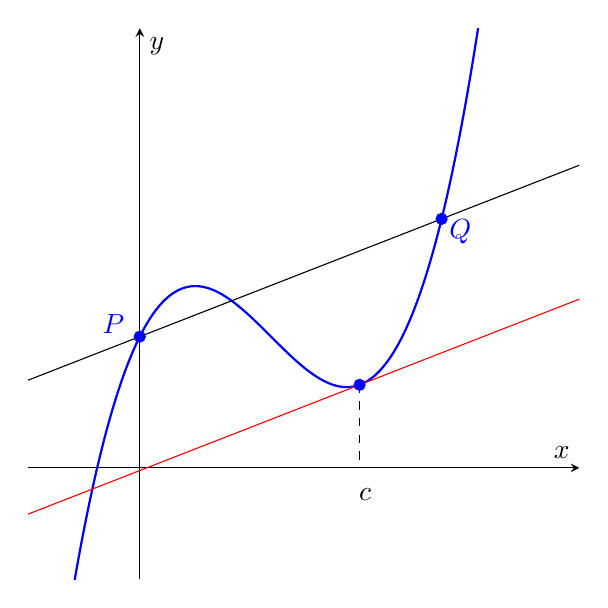
\begin{tikzpicture}
        \begin{axis}[
            xlabel=$x$,
            ylabel=$y$,
            axis equal,
            axis lines=middle,
            enlargelimits,
            xmax=3,
            xmin=-0.5,
            ymax=3,
            ymin=-0.5,
            xtick={0},
            ytick={0},
            scale only axis, 
            height=7cm, 
            width=7cm]
            \addplot [blue, thick, domain=-0.5:4, samples=1000] {(x-1)^3-(x-1)+1};
            \addplot [thin] {(+2.3+0.897*x)/2.3};
            \addplot [thin, red] {(-0.04762212198879534+0.897*x)/2.3};
            \addplot [only marks, blue] coordinates {
                (0,1) (2.3,1.897) (1.6750935416018717,0.6325812107948185)
            };
            \node at (-0.2,1.0958693092551806) {\textcolor{blue}{$P$}};
            \node at (2.4423312975392614,1.7967595468638561) {\textcolor{blue}{$Q$}};
            \node at (1.7167130769776808,-0.2) {$c$};
            \addplot [dashed, thin] coordinates {(1.6750935416018717,0.6325812107948185) (1.6750935416018717,0)};
        \end{axis}
    \end{tikzpicture}
\end{center}

Il teorema afferma che, sotto le ipotesi date, esiste un punto in cui la tangente è parallela alla secante.

\osservazione{
    La continuità su $ [a,b] $ è essenziale
}
\osservazione{
    La derivabilità in $ (a,b) $ è essenziale
}
\esempio[(controesempio)]{
    Sia $ f(x)=|x| $, $ f $ continua su $ [-1, 1] $, ma $ f $ non è derivabile in $ (-1, 1) $. La secante $ s:y=1 $ ha pendenza $ 0 $, ma \[
        \forall\,c \in (-1, 1)\, c\neq 0\: f'(c)=\pm 1; \quad f'(0)=\nexists
    \]
}

\lemma[(Teorema di Rolle)]{ettoreciccino}{
    Sia $ f:[a,b]\to \R $, $ f $ continua su $ [a,b] $, $ f $ derivabile su $ (a,b) $, e sia $ f(a)=f(b) $.

    Allora \[
        \exists\, c \in (a,b)\,\tc\quad f'(c)=0
    \]
}

\dimostrazionelem{ettoreciccino}{
    Se $ f $ è continua su $ [a,b] $ 
    
    $\implies$ per il teorema di Weierstrass $ \exists $ $ x_m $, punto di minimo assoluto, e $ x_{M}  $ punto di massimo assoluto \[
        M=f(x_{M})\qquad m=f(x_{m} )
    \]
    Ci sono due casi:
    \begin{itemize}
        \item \underline{Caso 1}: $ x_{m} $ e $ x_{M}  $ cadono entrambi negli estremi, \[
            x_{M}=a\,\land\, x_{m}=b\qquad \lor \qquad x_{m}=a\,\land\, x_{M}=b    
        \]
        Allora \begin{multline*}
            M=f(x_{M} )=\\
            =f(b)=f(a)=\\
            =f(x_{m} )= m
        \end{multline*} 
        
        $\implies$ $ M=m $, ma allora $ f $ deve essere costante su tutto $ [a,b] $ 
        
        $\implies$ $ \forall\,x \in [a,b] $, $ f'(x)=0 $.
        \item \underline{Caso 2}: almeno uno tra $ x_{m}$, $ x_{M}  $ case in $ (a,b) $; assumiamo che sia $ x_{M} \in (a,b)$.
        
        $ x_{M} \in (a,b)  $, $ f $ derivabile in $ x_{M}  $ e $ x_{M}  $ punto di massimo 
        
        $\implies$ per il teorema di Fermat $ f'(x_{M} )=0 $.

        Poniamo $ c=x_M $ 
        
        $\implies$ $ f'(c)=0 $\qed
    \end{itemize}
}

\teorema{cauchteccociqui}{
    Siano $ f:g, [a,b]\to \R $, $ f, g $ continua su $ [a,b] $, $ f, g $ derivabili su $ (a,b) $ 

    Allora $ \exists $ $ c \in (a,b) $ tale che \begin{equation}
        \left(f(b)-f(a)\right)\,g'(c)=\left(g(b)-g(a)\right)\,f'(c)
    \end{equation}
}
\dimostrazione{cauchteccociqui}{
    Consideriamo $ x \in [a,b] $ e poniamo \[
        W(x)=\left(f(b)-f(a)\right)\,g(x)-\left(g(b)-g(a)\right)\,f(x)
    \]
    Si ha che $ W(x) $ è continua in $ [a,b] $ e derivabile in $ (a,b) $.
    \begin{gather*}
        W(a)=\left(f(b)-f(a)\right)\,g(a)-\left(g(b)-g(a)\right)\,f(a)\\
        W(b)=\left(f(b)-f(a)\right)\,g(b)-\left(g(b)-g(a)\right)\,f(b)
    \end{gather*}
    È facile vedere che $ W(a)=W(b) $, quindi $ W(x) $ soddisfa le ipotesi del teorema di Rolle, 
    
    $\implies$ $ \exists\, c \in (a,b) $ tale che $ W'(c)=0 $.

    Si noti che $ W'(x) $ è \[
        W'(x)=\parentesi{\text{numero}}{\left(f(b)-f(a)\right)}\,g'(x)-\parentesi{\text{numero}}{\left(g(b)-g(a)\right)}\,f'(x)
    \] 
    
    $\implies$ $ W'(c) $ è \[
        W'(c)=\left(f(b)-f(a)\right)\,g'(c)-\left(g(b)-g(a)\right)\,f'(c)=0
    \] 
    
    $\implies$ $ \exists $ $ c \in (a,b) $ tale che \begin{equation*}
        \left(f(b)-f(a)\right)\,g'(c)=\left(g(b)-g(a)\right)\,f'(c)\qedd
    \end{equation*}
}

\dimostrazione{lagrangeettorepre}{[Del Teorema di Lagrange]

    Se $ g'(x)\neq 0 $ in $ (a,b) $, allora per Rolle sarà $ g(a)\neq g(b) $ (per $ g $ che soddisfa le ipotesi di Cauchy). Se così non fosse, $ \exists\, c \in (a,b) $ tale che $ g'(c)=0 $, contraddizione.

    Allora, se $ g $ soddisfa le ipotesi di Cauchy e $ g'(x)\neq 0 $ in $ (a,b) $ 
    
    $\implies$ (per il teorema di Cauchy)  $ \exists $ $ c \in (a,b) $ tale che, considerando $ f(x) $ continua in $ [a,b] $ e derivabile in $ (a,b) $ \[
        \frac{f(b)-f(a)}{g(b)-g(a)}=\frac{f'(c)}{g'(c)}
    \]

    Sia ora $ g(x):= x $, $ g'(x)=1\neq 0 $. Allora si ha che $ \exists $ $ c \in (a,b)$ tale che \begin{gather}
        \frac{f(b)-f(a)}{g(b)-g(a)}=\frac{f'(c)}{g'(c)}\\
        \frac{f(b)-f(a)}{b-a}=\frac{f'(c)}{1}\\
        f'(c)=\frac{f(b)-f(a)}{b-a}
    \end{gather} 
    Dimostrato il teorema di Lagrange.\qed
}
\begin{itemize}
    \item Il Teorema di Lagrange è importante e fondamentale;
    \item il Teorema di Rolle serve per dimostrare Lagrange;
    \item il Teorema di Cauchy è una generalizzazione del Teorema di Lagrange
\end{itemize}
Lo schema dimostrativo è \[
    \text{Rolle} \,\implies\, \text{Cauchy} \,\implies\, \text{Lagrange}
\]

\subsection{Test di Monotonia}

\teorema{testmonotonia}{
    Sia $ I $ intervallo aperto, $ I=(a,b) $, con $ a,b \in \R^{*} $.

    Sia $ f $ derivabile su $ I $, allora si ha:\begin{enumerate}
        \item [1.] $ \forall $ $ x \in I $, $ f'(x)=0 $ $ \iff $ $ f $ è costante su $ I$;
        \item [2.] $ \forall $ $ x \in I $, $ f'(x)\ge0 $ $ \iff $ $ f $ è crescente su $ I$;
        \item [2.1.] $ \forall $ $ x \in I $, $ f'(x)\le $ $ \iff $ $ f $ è decrescente su $ I$;
        \item [3] $ \forall $ $ x \in I $, $ f'(x)>0 $ $ \iff $ $ f $ è strettamente crescente su $ I$;
        \item [3.1.] $ \forall $ $ x \in I $, $ f'(x)<0 $ $ \iff $ $ f $ è strettamente decrescente su $ I$;
    \end{enumerate}
}
\dimostrazione{testmonotonia}{
    Procediamo con 2. $ f'(x)\ge 0 $
    \begin{itemize}
        \item [``$\impliedby$''] $ f $ crescente su $ I $ 
        
        $\implies$ $ \forall\, x_0, x \in I $ \[
            \frac{f(x)-f(x_0)}{x-x_0}\ge 0
        \]
        Allora \[
            \lim_{x\to x_0} \frac{f(x)-f(x_0)}{x-x_0}\ge 0 = f'(x_0)\ge 0
        \] per il teorema di permanenza del segno.
        \item [``$\implies$''] $ f'(x)\ge 0 $ su $ I $. Consideriamo $ x_1, x_2 \in I$, con $ x_1< x_2 $. Poiché $ f$ è derivabile su $ I $ 
        
        $\implies$ $ f $ è continua su $ [x_1, x_2] $ 
        
        $\implies$ Per il teorema di Lagrange $ \exists\, c \in (x_1,x_2) $ tale che \begin{align*}
            &\parentesi{\ge 0}{f'(c)}=\frac{f(x_2)-f(x_1)}{x_2-x_1}\\
            \implies &\frac{f(x_2)-f(x_1)}{\parentesi{>0}{x_2-x_1}}\ge 0\\
            \implies &f(x_2)-f(x_1)\ge 0\\
            \implies &f(x_2)\ge f(x_1)
        \end{align*} 
        
        $\implies$ $ f $ è crescente su $ I $.\qed
        
    \end{itemize}
}